\documentclass[11pt, compress, tikz]{beamer}

\usepackage{preamb}
\graphicspath{{./../doc/_images/}{./image_logi/}}

%%%%%%%%%%%%%%%%%%%%%%%%%%%%%%%%%% Styling for the beamer %%%%%%%%%%%%%%%%%%%%%%%%%%%%%%%%
%%%%%%%%%%%%%%%%%%%%%%%%%%%%%%%%%%%%%%%%%%%%%%%%%%%%%%%%%%%%%%%%%%%%%%%%%%%%%%%%%%%%%%%%%%

\setbeamertemplate{navigation symbols}{} 
\usetheme{Warsaw}

\setbeamertemplate{theorem begin}{{
\inserttheoremheadfont
\inserttheoremname
\inserttheorempunctuation
}}

\setbeamertemplate{theorem end}{}
\newtheorem{proposition}[theorem]{Proposition}

\theoremstyle{definition}
\newtheorem{mydef}[theorem]{Définition}
\makeatletter

%\captionsetup[figure]{labelformat=empty}
\definecolor{beamer@blendedpurp}{rgb}{0.41, 0.16, 0.38}
 % 0.8,0.2,0.3 rouge carmin presque rose assez élégant avec rgb
 %235 77 77 corail
 % .75 ,.2,.2 rouge clair  


\setbeamercolor{structure}{fg=beamer@blendedpurp}
\setbeamercolor*{palette quaternary}{fg=black,bg=white!80!gray } %bg=couleur à gauche header back
\makeatother
%\setbeamercolor{section in head/foot}{} no touch en fait casse tout
%\setbeamercolor{subsection in head/foot}{fg=black,bg=gray!30} idem 

\makeatletter
\defbeamertemplate*{footline}{shadow theme}
{%
  \leavevmode%
  \hbox{\begin{beamercolorbox}[wd=.5\paperwidth,ht=2.5ex,dp=1.125ex,leftskip=.3cm,rightskip=.3cm plus1fil]{title in head/foot}%
    \usebeamerfont{title in head/foot}\insertshorttitle%
  \end{beamercolorbox}}%
  \begin{beamercolorbox}[wd=.5\paperwidth,ht=2.5ex,dp=1.125ex,leftskip=.3cm plus1fil,rightskip=.3cm]{author in head/foot}%
    \usebeamerfont{author in head/foot}\hfill\insertframenumber\,/\,\inserttotalframenumber
  \end{beamercolorbox}%
  \vskip0pt%
}

%\setbeamertemplate{section in toc}{\textcolor{structure.fg}{$\blacktriangleright$}\hspace{1.2 em}~\inserttocsection \\}

%\setbeamertemplate{section in toc}{\inserttocsectionnumber.~\inserttocsection}
\setbeamercolor*{section in toc}{fg=black}
\setbeamercolor*{enumerate item}{fg=black}
\setbeamercolor*{enumerate subitem}{fg=black}
\newcommand*{\rom}[1]{\expandafter\@slowromancap\romannumeral #1@}
\makeatother

%%%%%%%%%%%%%%%%%%%%%%%%%%%%%%%%%%%%%%%%%%%%%%%%%%%%%%%%%%%%%%%%%%%%%%%%%%%%%%%%%
%%%%%%%%%%%%%%%%%%%%%%%%%%%%%%%%%% end styling beamer %%%%%%%%%%%%%%%%%%%%%%%%%%%


\title{Package chaoseverywhere}
\subtitle{Software development HMMA238}
\author{\vspace{-1.5cm}Lefort Tanguy, Coiffier Ophélie and Gaizi Ibrahim}
\date{\vspace*{-2cm}06-2020}
\institute[Montpellier University]{University of Montpellier}
\titlegraphic{%
  \makebox[0.9\paperwidth]{%
    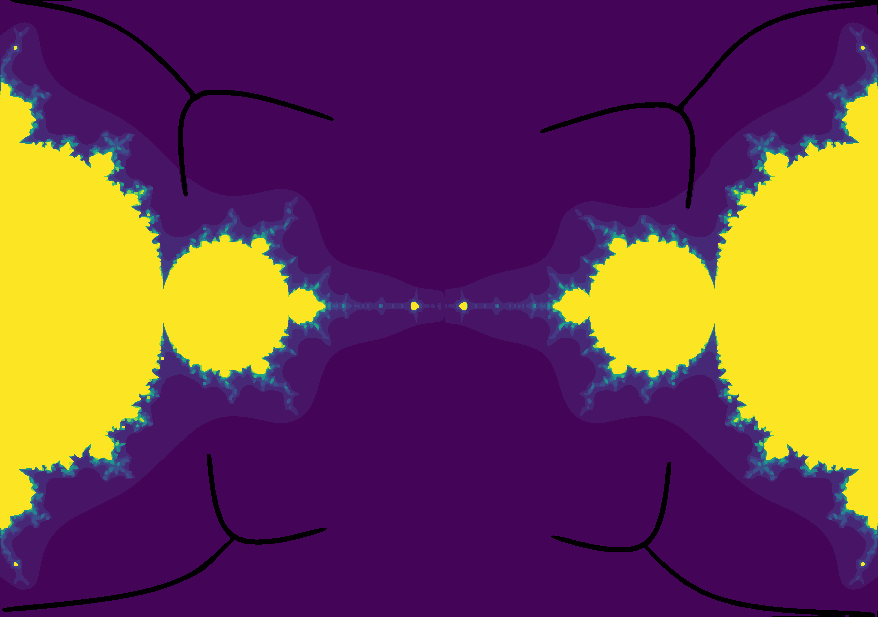
\includegraphics[scale=.2]{logo1_f.pdf}%
    \hfill%
    
\includegraphics[scale=.1]{logo_univ.pdf}%
    \hspace{.25cm}
  }%
}

\begin{document}

{
\def\mytitleframe{\bgroup
\makeatletter
\setbeamertemplate{footline}
{%
  \leavevmode%
  \hbox{\begin{beamercolorbox}[wd=.5\paperwidth,ht=2.5ex,dp=1.125ex,leftskip=.3cm,rightskip=.3cm plus1fil]{title in head/foot}%
    \usebeamerfont{title in head/foot}\insertshorttitle%
  \end{beamercolorbox}}%
  \begin{beamercolorbox}[wd=.5\paperwidth,ht=2.5ex,dp=1.125ex,leftskip=.3cm plus1fil,rightskip=.3cm]{author in head/foot}%
    \usebeamerfont{author in head/foot}%\hfill\insertframenumber\,/\,\inserttotalframenumber
  \end{beamercolorbox}%
  \vskip0pt%
}
\maketitle
\egroup
\addtocounter{framenumber}{-1}
}
\makeatother
	\mytitleframe
}


\section*{Contents}
\setbeamertemplate{background}{
   \tikz\node[opacity=0.2] at (current page.center) {
   					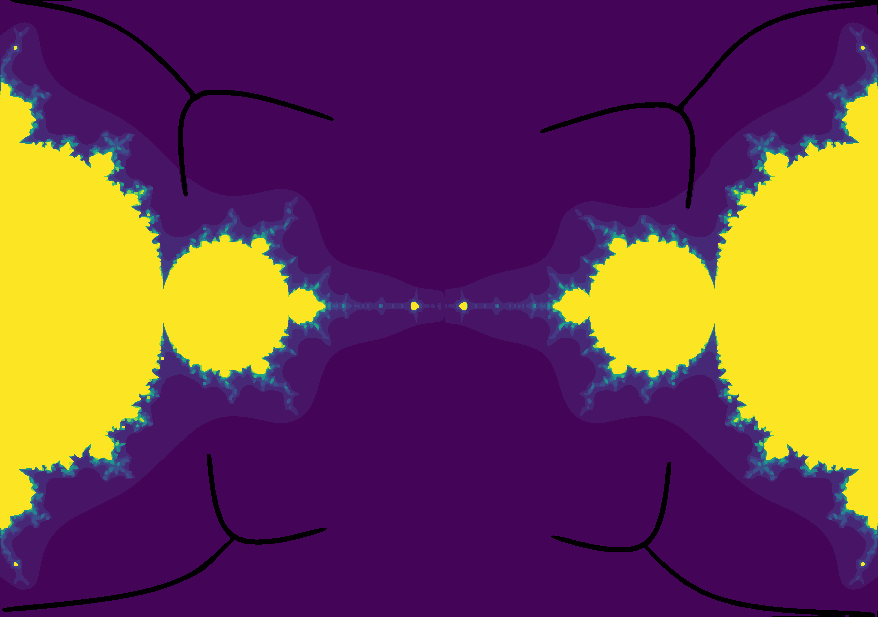
\includegraphics[trim = 1.1cm 0cm 0cm 0cm]{logo1_f.pdf}};}
\begin{frame}
\frametitle{Table of contents}
  \tableofcontents
\end{frame}      
\setbeamertemplate{background}{}


\section{Chaoseverywhere}
\subsection{Introduction}
\begin{frame}[fragile]{Chaoseverywhere}
Python3 package : \href{https://github.com/tanglef/chaoseverywhere}{\beamergotobutton{Github chaoseverywhere}}
%
\begin{minted}{python}
>>> import chaoseverywhere as chaos
\end{minted}
Includes $2$ main themes:
\begin{enumerate}[label=$\bullet$]
    \item the Manldebrot set,  %
    \item the logistic map. %
\end{enumerate}
\begin{block}<2>{Specific dependencies}
\begin{enumerate}[label=\ding{51}]
\item FFMPEG
\item Mayavi
\end{enumerate}
\end{block}
\end{frame}

\subsection{Generalities}
\begin{frame}[fragile]{Generalities}
Our subject deals with 2 mathematical objects :
\begin{block}{\textbf{Fractal}}
    It has a self-similarity at different scale.
\end{block}
\begin{block}{\textbf{Chaos}}
It is the behavior of the dynamic systems which are very sensitives at the initial conditions.
\end {block}
\end{frame}

\section[Logistic map]{The logistic map}
\subsection{The map}

\begin{frame}[fragile]{The logistic map: the cobweb diagram}
\vspace{-.25cm}
\begin{block}{Map formula}
\[x_{n+1} = rx_{n}(1-x_{n})\]
\end{block}
\vspace{-.3cm}

\begin{onlyenv}<1>
\begin{minted}{python}
>>> chaos.logistic_draw(x0=0.01, r=1.6, 50, 100)
\end{minted}
\end{onlyenv}

\begin{onlyenv}<2>
\begin{minted}{python}
>>> chaos.logistic_draw(x0=0.01, r=3.45, 50, 100)
\end{minted}
\end{onlyenv}

\begin{onlyenv}<3>
\begin{minted}{python}
>>> chaos.logistic_draw(x0=0.01, r=3.6, 50, 100)
\end{minted}
\end{onlyenv}
\begin{columns}
          \column{0.60\linewidth}
             \begin{onlyenv}<1-3>
             \vspace{-1.2cm}
  \begin{center}
    \includegraphics<1>[clip,scale=0.5, trim={.5cm 0 1.5cm 1.4cm}]{logistic_map1.pdf}
    \includegraphics<2>[clip,scale=0.5, trim={.5cm 0 1.5cm 1.4cm}]{logistic_map2.pdf}
    \includegraphics<3>[clip,scale=0.5, trim={.5cm 0 1.5cm 1.4cm}]{logistic_cobweb.pdf}
  \end{center}
\end{onlyenv}
             
           \column{0.40\linewidth}
           \vspace{-1.2cm}
           \begin{enumerate}[label=$\bullet$]
               \item<1-> $1 < r \leq 3 $: one point of convergence
               \item<2-> $3 < r \leq 3.57$ : oscillations between several values
               \item<3-> $r > 3.57$ : chaotic behavior
           \end{enumerate}
         \end{columns}

           
\end{frame}

\subsection{Bifurcation diagram}
\begin{frame}{Bifurcation diagram}
A summary of the logistic map: the bifurcation diagram
\begin{center}
    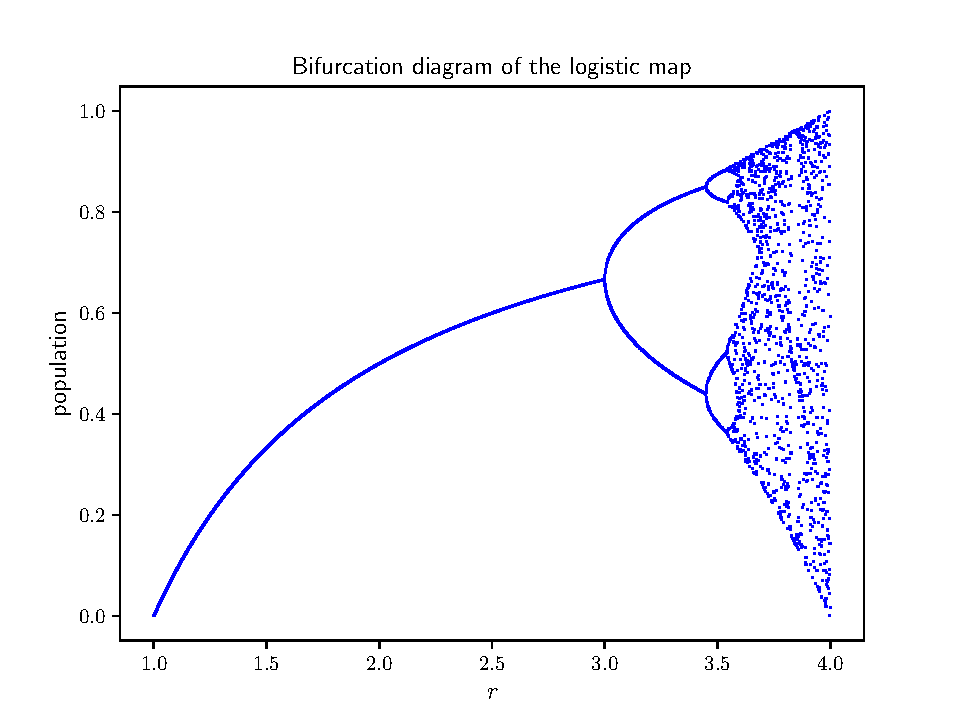
\includegraphics[scale=0.6]{bifurcation.pdf}
\end{center}
\end{frame}



\section[Mandelbrot]{The Mandelbrot set}
\subsection{Definition and caracteristics}


\begin{frame}{The Mandelbrot set: definition}



\begin{block}<1->{Definition}
The Mandelbrot set $\mathcal{M}$ is:
$$\mathcal{M}=\left\{ c\in\mathbb{C},\ (z_n)_n \text{ is bounded},\ \text{with } z_{n+1}=z_n^2+c,\ z_0=0\right\}.$$
\end{block}
\begin{block}<2->{Properties}
\begin{enumerate}[label=$\bullet$]
\item symmetry along the real axix,
\item contained in $\mathcal{D}((0,0),\, 2)$,
\item computed as a class object.
\end{enumerate}
\end{block}
\end{frame}

\subsection{Visualization}


\begin{frame}[fragile]{\emph{Mandel\_loop } method: Code}

\begin{minted}{python}
def mandel_loop(self, go_up=True, puiss=2):
    c = x + 1j * y
    z = np.zeros(c.shape)
    mandel = np.zeros(c.shape)
    for i in range(self.t_max):
        z = z ** puiss + c
        if go_up:
            mandel += 1 / float(2 + i) * 
                          (z * np.conj(z) > 4)
        else:
            mandel[z*np.conj(z) > 4] = i
    return(mandel)
\end{minted}

\end{frame}

\begin{frame}{\emph{Mandel\_loop } method: Output}
\begin{figure}
\begin{center}
    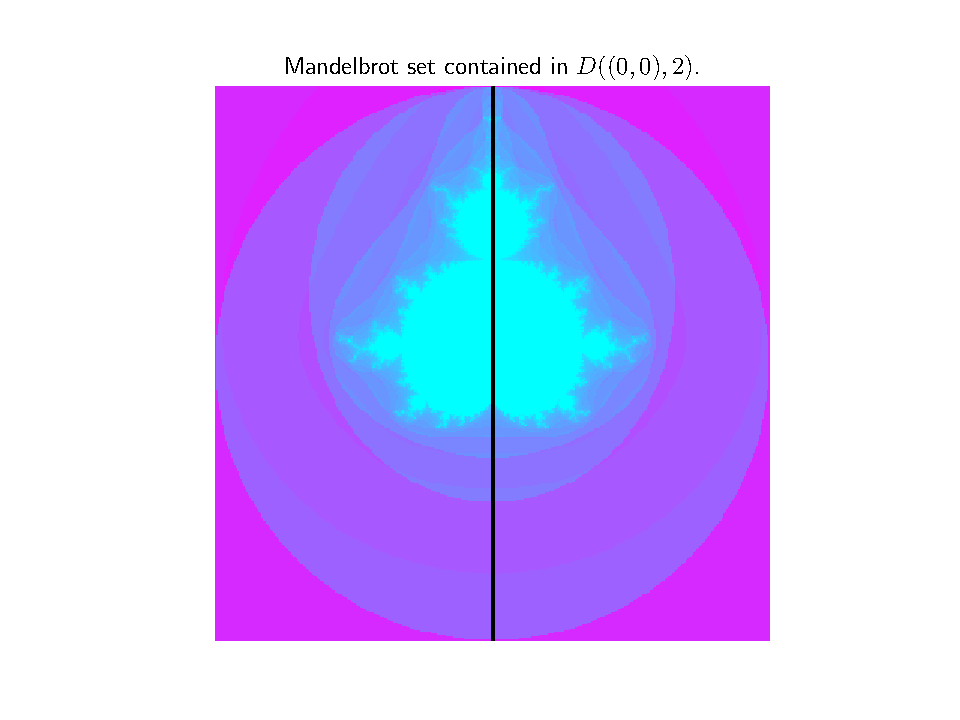
\includegraphics[scale=0.75, clip, trim={1cm 0 0 2cm}]{mandelbrot.pdf}
\end{center}
\end{figure}
\end{frame}


\section[Link]{Mandelbrot set and bifurcation diagram}

\begin{frame}[fragile]
\frametitle{Link between Mandelbrot set and bifurcation diagram}
If you're unable to display the animation, click here:
\href{https://www.youtube.com/watch?v=xYQbqML1eE4}{\beamergotobutton{Youtube}}
\begin{minted}[fontsize=\small]{python}
>>> chaos.connections()
\end{minted}

\IfFileExists{./img_connections/les_3-1.pdf}{\begin{figure}
					\animategraphics[controls,width=\linewidth,
					height=5.7cm,keepaspectratio]{30}{./img_connections/les_3-}{1}{360}
     				\end{figure}
     					}{\begin{center}
     						\begin{mybox}
     						\centering
     						\Large{Please click on the link above to see one \\
     													 wonderful animation!}
     						\end{mybox}
						\end{center}     				
     					}

\end{frame}

\section[]{Conclusion}
\begin{frame}{Conclusion}
\begin{center}
We have learnt how to:
\end{center}
\newtcolorbox{box2}{colback=purple!5!white,colframe=violet!80!black}
\begin{box2}{
\begin{enumerate}[label=$\bullet$]
\item illustrate \textbf{a chaotic} behavior with the logistic map and the bifurcation diagram,
\item represent the \textbf{Mandelbrot set} from different point of views,
\item see the \textbf{link} between these three objects.
\end{enumerate}}
\end{box2}
\begin{center}
Some possible upgrades are:
\end{center}
\begin{box2}{
\begin{enumerate}[label=\ding{42}]
\item other chaotic objects: Lorentz attractors (differential equations point of view)
\item mutli-threading for each quadrants of $\mathcal{M}$ for efficiency.
\end{enumerate}}
\end{box2}
\end{frame}  

\begin{frame}{Mandelbrot transformation}
\centering
\textit{\textbf{Thank you}}
\begin{center}
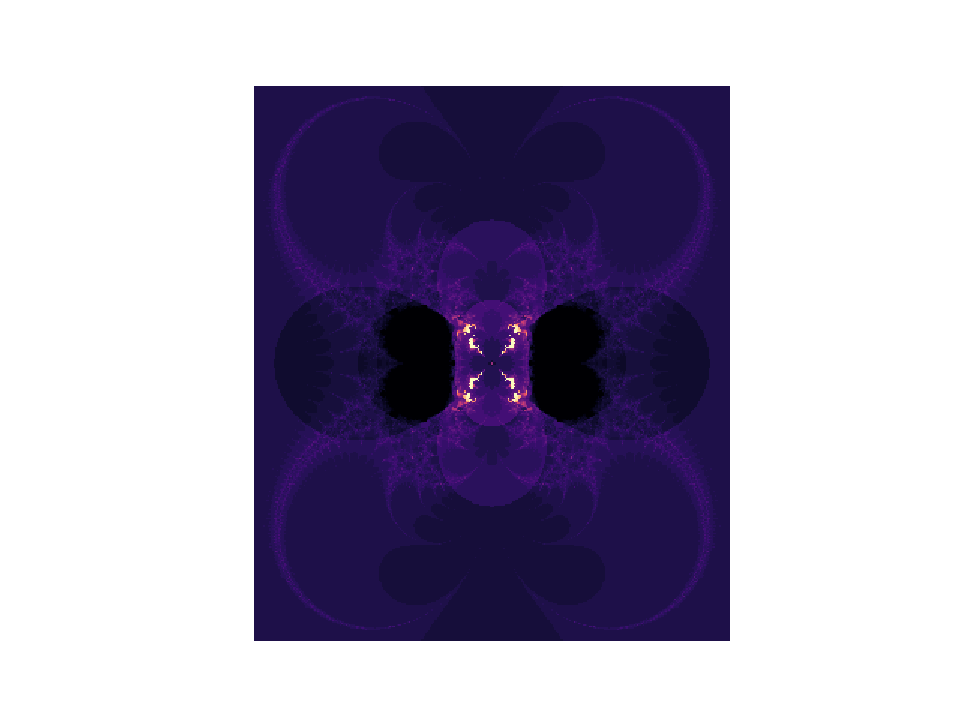
\includegraphics[scale=0.4, width=10cm, clip, trim={0 0 0 1cm}]{transformation.pdf}
\end{center}
\vspace{-1cm}
For more informations: \href{https://github.com/tanglef/chaoseverywhere}{\beamergotobutton{Github chaoseverywhere}}\href{https://chaoseverywhere.readthedocs.io/en/latest}{\beamergotobutton{Documentation chaoseverywhere}}
\end{frame}
\end{document}
